\documentclass[notitlepage, 11pt]{article}
\usepackage[english]{babel}           % LANGEUAGE=ENGLISH, UTF-8
\usepackage[utf8]{inputenc}
\usepackage[T1]{fontenc}
\usepackage{amsmath}                  % ALL MATH FEATURES
\usepackage{graphicx}                 % GRAPHICS                  
\usepackage{float}                    % IMPROVED FIGURE POSITIONING
\usepackage[labelsep=period,labelfont=bf]{caption} % IMPROVED CAPTIONS
\usepackage{url}                      % WRITE URLS
\usepackage{tikz}                     % MAKE TIKZ VECTOR GRAPHICS
\usepackage{tocloft}                  % CONTROL TABLE OF CONTENTS
\usepackage[authoryear,round]{natbib} % REFERENCES
\usepackage{apalike}
\usepackage{pdflscape}                % USE LANDSCAPE MODE
\usepackage{listing}                  % WRITING CODE AND ALGORITHMS
\usepackage{algpseudocode}            
%\usepackage{algorithm}  
%\usepackage{authblk}
\usetikzlibrary{decorations.pathreplacing}

\renewcommand{\familydefault}{lmr}           % SET DOCUMENT FONT
\makeatletter                         
\renewcommand{\section}{\@startsection       % SECTION
        {section}
        {2ex}
        {0mm}
        {1.2\baselineskip}
        {\baselineskip}
        {\centering\normalsize}}
\renewcommand{\subsection}{\@startsection    % SUBSECTION
        {subsection}
        {2ex}
        {0mm}
        {.8\baselineskip}
        {.5\baselineskip}
        {\bfseries\normalsize}}
\renewcommand{\subsubsection}{\@startsection % SUBSUBSECTION
        {subsubsection}
        {2ex}
        {0mm}
        {.5\baselineskip}
        {0mm}
        {\it\bfseries\normalsize}}    
\makeatother

\title{Simulating dark matter in an expanding universe using a parallel multigrid method}
\author{{\em Otto Hannuksela} \and {\em Janne Lampilahti}}
\date{\today}

\floatstyle{plaintop}
\newfloat{algorithm}{bpht}{alg}
\floatname{algorithm}{Algortihm}

\begin{document}
\maketitle
\section*{INTRODUCTION}
Dark matter appears to be the dominant form of matter in the universe. While no direct observations of dark matter exist, it has been observed indirectly through its gravitational interaction with visible matter and radiation. The effect of dark matter on structure formation in the universe is the subject of an increasing scientific interest and a useful tool in the search for possible candidates of dark matter. Current progress in the investigation of structure formation is mainly driven by advances in computational methods and capabilities. 

In this work we simulate dark matter, neglecting baryonic matter, by using a particle based method and solving the Poisson's equation of gravity in a comoving frame of reference. The software used is {\em Uintah}, a parallel partial differential equation solver on an adaptively refined multigrid.
\section*{THEORY}
The gravitational potential $\phi$ is given by the Poisson's equation of gravity
\begin{equation}
\nabla^2 \phi = 4\pi G \rho
\end{equation}
where $\rho$ is the mass density. In our case we have a set of massive particles. The corresponding force field can be solved from the gradient
\begin{equation}
\mathbf{F} = -\nabla \phi.
\end{equation}
A new position and velocity for the particles after a time step $dt$ can be solved from Newton's equation of motion.
\begin{align}
\mathbf{v}(t+dt) &= \int_{t}^{t+dt}\frac{\mathbf{F}(t')}{m}dt' +  \mathbf{v}(t)\\
\mathbf{x}(t+dt) &= \int_{t}^{t+dt}\mathbf{v}(t')dt' +  \mathbf{x}(t)
\end{align}

\section*{METHODS}
The simulation is set up with respect to an adaptively refined three dimensional grid that supports particles (Fig. \ref{fig:grid}).
\begin{figure}[H]
\centering
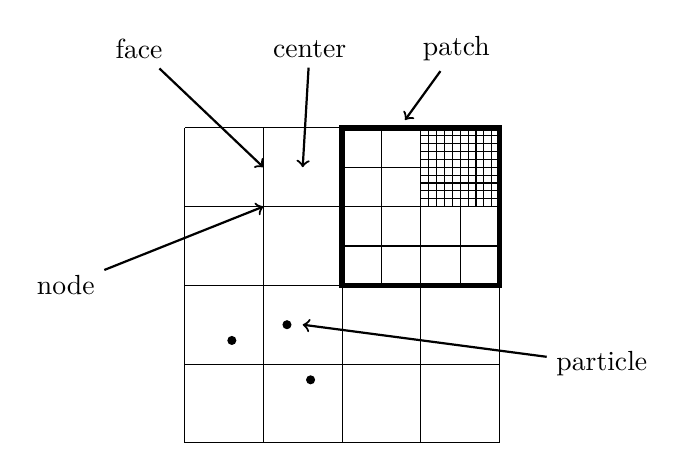
\begin{tikzpicture}
\node [anchor=west] (node) at (-1,3) {node};
\node [anchor=west] (face) at (0,6) {face};
\node [anchor=west] (center) at (2,6) {center};
\node [anchor=east] (patch) at (5,6) {patch};
\node [anchor=east] (particle) at (7,2) {particle};
\draw (1,1) grid (5,5);
\draw [step=0.5] (3,3) grid (5,5);
\draw [step=0.1] (4,4) grid (5,5);
\draw [line width=2] (3,3) rectangle (5,5);
\draw [->,thick] (node) -- (2,4);
\draw [->,thick] (face) -- (2,4.5);
\draw [->,thick] (center) -- (2.5,4.5);
\draw [->,thick] (patch) -- (3.8,5.1);
\draw [->,thick] (particle) -- (2.5,2.5);
\draw [fill] (2.3,2.5) circle [radius=0.05];
\draw [fill] (2.6,1.8) circle [radius=0.05];
\draw [fill] (1.6,2.3) circle [radius=0.05];
%\draw [black,decorate,decoration={brace,amplitude=5pt},
%   xshift=5pt,yshift=0pt] (5,5)  -- (5,3)
%   node [black,midway,below=-8pt,xshift=20pt] {AMR};
\end{tikzpicture}
\caption{A two dimensional view of the grid with its various components and properties shown.}
\label{fig:grid}
\end{figure}
The overall algortihm is expressed in Algortihm \ref{alg:main}.
\begin{algorithm}[H]
\hspace{0.1\textwidth}\parbox{.8\textwidth}{
\-\hspace{0ex}set boundary conditions\\
\-\hspace{0ex}set initial $\mathbf{x}_p$, $\mathbf{v}_p$ and $m_p$ for particles $p$\\
\-\hspace{0ex}calculate initial $\rho$\\
\-\hspace{0ex}set initial guess for $\phi$\\
\-\hspace{0ex}{\bf loop}\\
\-\hspace{4ex}solve $\phi$ using SOR algorithm\\
\-\hspace{4ex}calculate $\mathbf{F}=-\nabla \phi$\\
\-\hspace{4ex}{\bf for} every particle $p$ {\bf do}\\
\-\hspace{8ex}$\mathbf{v}_p(t+\Delta t) = (\mathbf{F}_p/m)\Delta t + \mathbf{v}_p(t)$\\
\-\hspace{8ex}$\mathbf{x}_p(t+\Delta t) = \mathbf{v}_p(t)\Delta t + \mathbf{x}_p(t)$\\
\-\hspace{4ex}{\bf end for}\\
\-\hspace{4ex}calculate $\rho$\\
\-\hspace{4ex}$t\leftarrow t+\Delta t$\\
\-\hspace{0ex}{\bf end loop}}
\caption{Main program.}
\label{alg:main}
\end{algorithm}

The Poisson's equation is solved with the successive over relaxation (SOR) algortihm (see Alg. \ref{alg:SOR}). The potential $\phi$ is solved at each node. In the calculation of the potential gradient we obtain the potential values near the particles by interpolation and then calculate the gradient by numerical differentiation. For exmaple at the $p$th particle the gradient is calculated in the $x$ direction as
\begin{equation}
(\nabla \phi)(x_p)=\frac{\phi(x_p+dx)-\phi(x_p-dx)}{2dx},
\end{equation}
where $x_p$ is the particle's $x$ coordinate and $dx$ is a small distance. 

The particle velocity and position are evolved over a small time step $dt$, assuming that the force remains constant. After this the particle masses are again interpolated back to the nodes to obtain a new mass density $\rho$.

\begin{algorithm}[H]
\hspace{0.1\textwidth}\parbox{.8\textwidth}{
\-\hspace{0ex}{\bf function} SOR($\phi$, tolerance, max\_iterations)\\
\-\hspace{4ex}{\bf for} $n = 0,1,\ldots\mbox{max\_iterations}$ {\bf do}\\
\-\hspace{8ex}error $\sigma\leftarrow 0$\\
\-\hspace{8ex}{\bf for} every node $\phi_{i,j,k}$\\
\-\hspace{12ex}$\phi_{i,j,k}^{(n+1)} \leftarrow (1-\omega)\phi_{i,j,k}^{(n)} + \frac{\omega}{6} (\phi_{i+1,j,k}^{(n)} +\phi_{i-1,j,k}^{(n)}+$\\
\-\hspace{12ex}$\phantom{\phi_{i,j,k}^{(n+1)} \leftarrow }\phi_{i,j+1,k}^{(n)}+ \phi_{i,j-1,k}^{(n)} + \phi_{i,j,k+1}^{(n)} + \phi_{i,j,k-1}^{(n)} +$\\
\-\hspace{12ex}$\phantom{\phi_{i,j,k}^{(n+1)} \leftarrow} h^3\rho_{i,j,k})$\\
\-\hspace{12ex}update $\sigma$\\
\-\hspace{8ex}{\bf end for}\\
\-\hspace{8ex}{\bf if} $\sigma \leq $ tolerance, {\bf break}\\
\-\hspace{4ex}{\bf end for}\\
\-\hspace{4ex}{\bf return} $\phi$\\
\-\hspace{0ex}{\bf end function}}
\caption{Calculating potential $\phi$ using the SOR algorithm.}
\label{alg:SOR}
\end{algorithm}


\section*{IMPLEMENTATION}
\subsection*{Uintah}
% describe uintah
\subsection*{Program}
\section*{RESULTS}
% visit figure:
% initial vs final condition
% mp4 movie...
\section*{CONCLUSIONS}
% what should we do next?

%\renewcommand{\refname}{REFERENCES} 
%\bibliography{NameOfReferenceFile}{}
%\bibliographystyle{plainnat}
\end{document}
